
\documentclass[lnbip]{svmultln}
\usepackage{makeidx}
\usepackage{tcolorbox}
\usepackage{multirow}
\usepackage{amsmath}
\usepackage[utf8x]{inputenc}
\usepackage[pdfencoding=auto]{hyperref}
\usepackage{listings}[language=R]
\usepackage{xcolor}
\usepackage{enumitem}
\graphicspath{ {./images/} }

\definecolor{codegreen}{rgb}{0,0.6,0}
\definecolor{codegray}{rgb}{0.5,0.5,0.5}
\definecolor{codepurple}{rgb}{0.58,0,0.82}
\definecolor{backcolour}{rgb}{0.95,0.95,0.92}

\lstdefinestyle{mystyle}{
    backgroundcolor=\color{backcolour},   
    commentstyle=\color{codegreen},
    keywordstyle=\color{magenta},
    numberstyle=\tiny\color{codegray},
    stringstyle=\color{codepurple},
    basicstyle=\ttfamily\footnotesize,
    breakatwhitespace=false,         
    breaklines=true,                 
    captionpos=b,                    
    keepspaces=true,                 
    numbers=left,                    
    numbersep=5pt,                  
    showspaces=false,                
    showstringspaces=false,
    showtabs=false,                  
    tabsize=2
}
\lstset{style=mystyle}
\lstset{language=R}

\makeindex

\begin{document}
\mainmatter
\title{Probabilidade Bayesiana}

\author{Flávio Luiz Seixas\inst{1}}
\institute{Instituto de Computação\\
\email{fseixas@ic.uff.br},
\texttt{http://www.ic.uff.br/~fseixas}}

\maketitle

\section{Paradigmas Frequentista e Bayesiano}

O paradigma frequentista admite a probabilidade num contexto restrito a fenômenos que podem ser medidos por frequências relativas. O paradigma Bayesiano entende-se que a probabilidade é uma medida racional e condicional de incerteza. Uma medida do grau de plausibilidade de proposições quaisquer, as quais não precisam necessariamente estar associadas a fenômenos medidos por frequência relativa. Por exemplo, no paradigma Bayesiano admite-se falar da probabilidade de extinção de uma espécie, o que não seria admissível sob o paradigma frequentista.

A inferência estatística é o processo formal utilizado para fazer afirmações genéricas com base em informações parciais. Essas afirmações sáo probabilísticas pois se caracterizam por incluir componentes de incerteza.

Na perspectiva bayesiana, a inferência estatística sobre qualquer quantidade de interesse é descrita como a modificação que se processa nas incertezas à luz de novas evidências.

A conceituação frequentista admite falar em probabilidades somente no contexto de frequências relativas. Em contraste, na conceituação bayesiana, probabilidades quantificam as plausibilidades de proposições ou eventos. Ao atribuir plausibilidades diferenciadas a proposições, a formalização bayesiana de probabilidade estende a lógica dedutiva, restrita a classificar proposições em verdadeiras (probabilidade igual a 1) ou falsas (probabilidade igual a zero), para um conjunto de possibilidades entre estes dois extremos.

O rápido crescimento do uso do paradigma bayesiano em ciências aplicadas ao longo das últimas décadas foi facilitado pelo surgimento de vários programas para efetuar as computações estatísticas. Entre esses, destaca-se o R (programa de livre distribuições e de código aberto).

\section{As Regras de Probabilidade}

A probabilidade será um número real e função de dois argumentos: o evento incerto $E$ e a premissa $H$. Utilizaremos o símbolo $Pr(E|H)$ lido como probabilidade de $E$ dado que $H$ é fato, ou a probabilidade de $E$ condicionada ao fato $H$.

\begin{tcolorbox}[colback=blue!5,colframe=blue!75!black,title=A Lei da convexidade]
    A probabilidade de um evento qualquer $E$, condicionado a $H$ é um número real no intervalo $[0,1]$
    \begin{equation}
        0<Pr(E|H)<1
    \end{equation}
\end{tcolorbox}

\begin{tcolorbox}[colback=blue!5,colframe=blue!75!black,title=A Lei da adição]
    Se $E_1$ e $E_2$ são eventos exclusivos sob $H$, então a probabilidade da união lógica de $E_1 + E_2$ é igual a soma aritmética das suas probabilidades individuais condicionadas a $H$.
    \begin{equation}
        Pr(E_1 + E_2 | H) = Pr(E_1|H) + Pr(E_2|H)
    \end{equation}
\end{tcolorbox}

\begin{tcolorbox}[colback=blue!5,colframe=blue!75!black,title=A Lei do produto]
    Se $E_1$ e $E_2$ são eventos quaisquer então a probabilidade do produto lógico $E_1 E_2$ condicionado a $H$ é o produto da probabilidade de $E_1$ condicionado a $H$ multiplicado pela probabilidade de $E_2$ condicionado a $E_1 H$
    \begin{equation}
        Pr(E_1 E_2 | H) = Pr(E_1|H) \cdot Pr(E_2|E_1 H)
    \end{equation}
\end{tcolorbox}

Nos casos em que estamos tratando de eventos independentes, a lei do produto pode ser reescrita como:
\begin{equation}
    Pr(E_1 E_2 | H) = Pr(E_1|H) \cdot Pr(E_2|H)
\end{equation}

\section{O Teorema de Bayes}

Mutas propriedades do cálculo de probabilidades podem ser deduzidas a partir das três leis básicas indicadas na seção anterior. Depois teoremas adicionais merecem especial destaque, o Teorema da Probabilidade Total e o Teorema de Bayes.

\begin{tcolorbox}[colback=blue!5,colframe=blue!75!black,title=Teorema da Probabilidade Total]
    Seja ${E_1; j=1, ..., m}$ um conjunto de $m$ eventos exclusivos e exaustivos sob $H$, e seja $A$ outro evento qualquer. Então $Pr(A|H)$ pode ser reescrito estendendo a conversa para a inclusão dos $E_j$.
    \begin{equation}
        Pr(A|H) = \sum_{j=1}^{m}{Pr(A|E_j H) \cdot Pr(E_j|H)}
    \end{equation}
\end{tcolorbox}

\begin{tcolorbox}[colback=blue!5,colframe=blue!75!black,title=Teorema de Bayes]
    Sejam $E$ e $F$ dois eventos quaisquer e $Pr(E|H)>0$, então:
    \begin{equation}
        Pr(F|E H) = \frac{Pr(E|F H) \cdot Pr(F|H)}{Pr(E|H)}
    \end{equation}
\end{tcolorbox}

\subsection{Exemplo}

Um estudo de uma mamografia no diagnóstico de câncer é apresentado na Tabela~\ref{tab:tab1}. Os dados foram obtidos experimentalmente sobre a efetividade do exame na detecção de um tumor de mama maligno ou benigno. Por exemplo, se um tumor é maligno $Ca$, a probabilidade de que o exame resulte positivo é $Pr(Pos | Ca) = 0,792$, ou seja, 79,2\%. De forma similar temos $Pr(Neg | Ca') = 0,904$ como a probabilidade de que o exame resulte negativo se o tumor não é maligno $(Ca')$. Os percentuais para faltos positivos e falsos negativos são 9,6\% e 20,8\%, respectivamente.

\begin{table}[h]
    \caption{Resultados dos testes de câncer de mamas}
    \label{tab:tab1}
    \center
    \begin{tabular}{ |c|c|c| } 
    \hline
    \multirow{2}{4em}{Resultado do teste} & \multicolumn{2}{|c|}{Realidade} \\
    & $Ca$ (Tumor maligno) & $Ca'$ (Tumor benigno) \\ 
    \hline
    $Pos$ (Positivo) & 0,792 & 0,096 \\ 
    $Neg$ (Negativo) & 0,208 & 0,904 \\ 
    \hline
    \end{tabular}
\end{table}

Com essa tabela, fez-se a seguinte pergunta: "Suponha que uma paciente pertença a uma população (mesmo grupo etário, hábito alimentar, etc.) na qual a incidência geral de câncer de mama é de 1\%. Detectado um nódulo no seio desta paciente, pede-se uma mamografia para avaliar a possibilidade de que se trate de um tumor maligno; o resultado é positivo. De posse deste conjunto de informações, qual é, em sua opinião, a probabilidade de tratar-se de um tumor maligno?"

Pelo Teorema de Bayes:
\begin{equation}
\begin{split}
Pr(Ca|Pos) & = \frac{Pr(Pos|Ca) \cdot Pr(Ca)}{Pr(Pos)} \\
& = \frac{Pr(Pos|Ca) \cdot Pr(Ca)}{P(Pos|Ca) \cdot P(Ca) + Pr(Pos|Ca') \cdot Pr(P(Ca')} \\
& = \frac{0,792 \cdot 0,01}{0,792 \cdot 0,01 + 0,096 \cdot 0,99} = 0,077
\end{split}
\end{equation}

Observe que a acurácia retrospectiva do exame $Pr(Pos|Ca)$ é diferente de acurácia preditiva $Pr(Ca|Pos)$. Na prática, a importância atribuída à alta probabilidade de um resultado positivo quando o tumor é de fato maligno, $Pr(Pos|Ca) = 0,792$ foi excessiva com relação a baixa probabilidade de incidência desse tipo de câncer $Pr(Ca)=0,01$. No contexto mais geral de investigação científica, o Teorema de Bayes expressa o mecanismo pelo qual hipóteses científicas e evidências empíricas são integrados.

Seja $F$ uma hipótese científica cuja probabilidade corrente é $Pr(F|H)$. Seja $E$ a evidência contida nos dados, experimentais ou observacionais, e cuja probabilidade sob a premissa $F$ é dada por $Pr(E|F,H)$. Então, se efetivamente foi observado $E$, o Teorema de Bayes permite calcular a probabilidade atualizada $Pr(F|E,H)$ da hipótese $F$. Portanto, a probabilidade atualizada de $F$ é composta pela sua probabilidade a priori, modificada pela acresção das novas evidências $E$ presentes nos dados.
\section{Variáveis aleatórias}

As variáveis aleatórias são de dois tipos. As discretas associadas a alguma contagem, e as contínuas que envolvem medições ou mesmo razões. A distinção é necessária para que as regras do cálculo das probabilidades sejam corretamente aplicadas a cada caso. Segue um resumo das propriedades e distinções dos principais modelos de probabilidades para variáveis aleatórias discretas e contínuas.

\subsection{Variáveis Aleatórias Discretas}

Uma variável aleatória discreta $X$ é uma função que associa as proposições de interesse a um conjunto enumerável (ou categórico, que pode ser nominal ou ordinal), não necessariamente finito, de valores. Se, por exemplo, $X$ caracteriza o número de amostras de sangue avaliadas antes do aparecimento de uma amostra que contém um vírus de interesse, então os possíveis valores para $X$ que caracterizam um conjunto infinito 0, 1, 2, ... já que náo existe um limite superior para delimitá-lo.

De modo geral, o valor $Pr(X = x_j | H)$ denota a massa de probabilidade no ponto $x_j$. Sobre o conjunto de todos os pontos plausíveis, ou seja, pontos com massa de probabilidade maior que zero, a Lei da adição garante que:

\begin{equation}
    \sum_{j}{Pr(X = x_j|H)} = 1
\end{equation}

A média ou valor esperado de $X$, $E(X)$, e a sua variância, $V(X)$, são definidas por:

\begin{equation}
\begin{split}
    E(X) = \sum_{j}{x_j Pr(X = x_j|H)} \\
    V(X) = \sum_{j}{(x_j - E(X))^2 Pr(X = x_j|H)}
\end{split}
\end{equation}

\subsection{Variáveis Aleatórias Contínuas}

Quando os possíveis valores de $X$ foram um subconjunto que compreende pelo menos um intervalo da escala de números reais, a variáveis aleatória é denominada contínua. Variáveis aleatórias contínuas são caracterizadas pela sua função distribuição cumulativa $F(x)$ que é definida para todo o número real $x \in (-\infty \infty)$.

\begin{equation}
    F(x) = Pr(X \leq x | H)
\end{equation}

A função densidade de probabilidade é definida por $f(x) = \frac{F(x)}{dx}$. A integração da densidade de probabilidade sobre os números reais é igual a 1, ou seja: $\int_{-\infty}^{\infty}{f(x) \cdot dx} - 1$.

A média e a variância de $X$ também são expressos em integrais:

\begin{equation}
\begin{split}
    E(X) = \int{x \cdot f(x) dx} \\
    V(X) = \int{(x - E(X))^2 \cdot f(x) dx}
\end{split}
\end{equation}
\section{Distribuições de Probabilidade}

Denomina-se de distribuição de probabilidade de alguma variável aleatória a regra geral que define a função de massa de probabilidade (variável discreta) ou de densidade de probabilidade (variável contínua) para a variável de interesse.

\subsection{Distribuições Discretas}

\subsubsection{Distribuição Uniforme Discreta Ud(a,b)}

\begin{equation}
    p(x) = \frac{1}{b-a+1}
\end{equation}

\subsubsection{Distribuição Binomial Bin(n,$\theta$)}

\begin{equation}
    p(x) = \begin{pmatrix} n\\x \end{pmatrix} \cdot \theta^x \cdot (1-\theta)^{n-x}
\end{equation}

\subsubsection{Distribuição Hipergeométrica Hip(M, N, n)}

\begin{equation}
    p(x) = \frac{\begin{pmatrix} M\\x \end{pmatrix} \cdot \begin{pmatrix} N-M\\n-x \end{pmatrix}}{\begin{pmatrix} N\\n \end{pmatrix}}
\end{equation}

\subsubsection{Distribuição de Poisson Poi($\mu$)}

\begin{equation}
    p(x) = \frac{e^\mu \mu^x}{x!}
\end{equation}

\subsubsection{Distribuição Binomial Negativa BinN(a,$\theta$)}

\begin{equation}
    p(x) = \frac{(a + x - 1)!}{x! (a-1)!} \cdot \theta^a(1-\theta)^x
\end{equation}

\subsection{Distribuição Contínua}

\subsubsection{Distribuição Uniforme U(c,d)}

\begin{equation}
    p(x) = \frac{1}{d-c}
\end{equation}

\subsubsection{Distribuição Beta($\alpha$, $\beta$)}

\begin{equation}
    p(x) = \frac{\Gamma(\alpha+\beta)}{\Gamma(\alpha) \Gamma(\beta)} \cdot x^{\alpha+1} (1-x)^{\beta-1}
\end{equation}

\subsubsection{Distribuição Beta Gerenalizada}

\subsubsection{Distribuição Exponencial}

\subsubsection{Distribuição Gama}

\subsubsection{Distribuição Gama Inversa}

\subsubsection{Distribuição Normal}

\subsubsection{Distribuição Student}

\subsection{Exemplo de códigos gerados no R}

\lstinputlisting[language=Octave]{code/graficos.r}

\section{Análise Bayesiana de Dados}

A inferência bayesiana consiste na construção de uma distribuição de probabilidade posterior via o Teorema de Bayes. Essa distribuição resulta da combinação de informações prévias, sumarizadas em uma distribuição denominada priori, com dados estatísticos descritos por algum modelo probabilístico e resumidos na função de verossimilhança.

A distribuição posterior é a forma mais completa de expressar o estado do conhecimento sobre o fenômeno investigado. Toda pergunta específica é respondida a partir da análise da distribuição posterior. Ela contém toda a informação necessária para a inferência.

Além disso, o processo é dinâmico. A distribuição posterior de hoje pode se transformar na priori em estudos futuros, caracterizando o elemento cumulativo de aquisição de informações.


\section{Redes Bayesianas}

Redes bayesianas sãp uma classe de modelos gráficos que permitem a representação de probabilidades condicionais entre um conjunto dado de variáveis aleatórias $X = {X_1,X_2,...X_p}$ como um grafo acíclico direto (DAG) $G = (V,A)$. Cada nó $v_i \in V$ corresponde a uma variável aleatória $X_i$.

As redes Bayesianas podem ser utilizadas para:
    
    \begin{itemize}
        \item Tomar decisões baseadas em probabilidades.
        \item Decidir quais evidências adicionais devem ser observadas, a fim de obter total conhecimento do domínio.
        \item Realizar uma análise sensitiva para entender quais aspectos do modelo tem maior impacto sobre determinadas variáveis.
        \item Explicar os resultados de uma inferência probabilística.
\end{itemize}
    
\subsection{Propriedades das Redes Bayesianas}

Um exemplo de DAG é mostrado na Figura~\ref{fig:fig75}. Nesse exemplo, a variável $Z$ é condicionada às variáveis $X$ e $Y$.

\begin{figure}[t]
    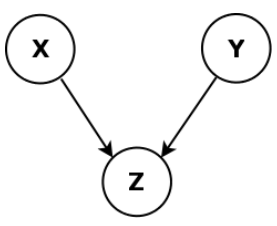
\includegraphics[width=4cm]{fig75.png}
    \centering
    \caption{Representação de probabilidades condicionais um grafo acíclioco direto (DAG).}
    \label{fig:fig75}
\end{figure}

Assim, uma rede Bayesiana consiste:

\begin{itemize}
    \item Um conjunto de variáveis e um conjunto de arcos ligando as variáveis;
    \item Cada variável possui um número limitado de estados mutuamente exclusivos;
    \item As variáveis e arcos formam um grafo dirigido e sem ciclos;
    \item Para cada variável $A$ que possui como pais $B_1, ..., B_n$, existe uma tabela de probabilidade condicional (TPC) $P(A|B_1, ..., B_m)$.
\end{itemize}

Uma rede Bayesiana é a representação de um domínio caso a condição de Markov seja satisfeita. A condição de Markov é definida dessa forma: suponha a distribuição de probabilidade conjunto das variáveis aleatórias em um conjunto de nós $V$ em um DAG $G = (V, E)$. Então, dizemos que $(G, P)$ satisfazem a condição de Markov se cada variável $X \in V, X$ é condicionalmente independente dos nós não descendentes dados os seus pais.

A condição de Markov afirma que as variáveis não-descendentes não fornecem informações adicionais sobre a variável em questão. Considerando $f_X$ e $Pa_X$ o conjunto de filhos e dos pais do nó $X$ respectivamente, e ainda $Pa_{F_{X}}$ como o conjunto dos pais dos descendentes diretos de $X$. O conjunto de nós formados pela união desses três conjuntos é denominado Markov Blanket (ver Figura~\ref{fig:fig76}).

\begin{figure}[t]
    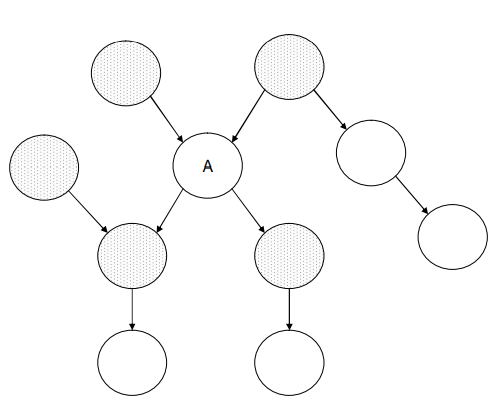
\includegraphics[width=8cm]{fig76.png}
    \centering
    \caption{Os nós preenchidos com cinza representam o conjunto de nós conforme critério Markov Blanket.}
    \label{fig:fig76}
\end{figure}

Se uma rede Bayesiana satisfaz a condição de Markov, então a sua distribuição de probabilidade conjunto é igual ao produto das probabilidades condicionais de todos os nós dado os valores de seus pais.

\begin{equation}
    Pr(X_1, ..., X_n) = \prod_{i=1}^{n}{Pr(X_i | pa(X_i))}
\end{equation}

Através das propriedades markovianas, podemos considerar que a variável aleatória é independente de outra se não existe entre as variáveis analisadas um grupo específico de variáveis, podendo ser um grupo de evidências. Nesse caso, surge o conceito de d-separação. Para defini-la, consideremos alguns tipos de conexões. Seja $X$, $Z$, e $Y$ variáveis de uma rede Bayesiana $(\xi, V)$, definimos alguns tipos de conexão:

\begin{enumerate}
    \item Se $X \rightarrow Z \rightarrow Y$. temos um relacionamento head-to-tail;
    \item Se $X \leftarrow Z \rightarrow Y$, temos um relacionamento tail-to-tail;
    \item Se $X \rightarrow Z \leftarrow Y$, temos um relacionamento head-to-head.
\end{enumerate}

\begin{figure}[t]
    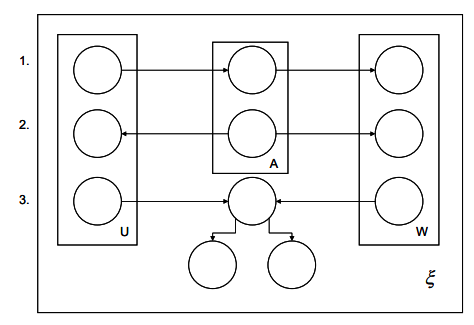
\includegraphics[width=8cm]{fig77.png}
    \centering
    \caption{A independência entre as variáveis aleatórias analisadas em relação ao tipo de conexão.}
    \label{fig:fig77}
\end{figure}

Dada a rede Bayesiana $(\xi, V)$, representada na Figura~\ref{fig:fig77}. Podemos definir $A \subset V$, sendo $X$ e $Y \in V - A$. Desta forma, para os casos 1 e 2, se consideramos que $Z \in A$, a variável $Z$ bloqueará o caminho entre $X$ e $Y$. Para o caso 3, se consideramos que $Z$ e seus descendentes $\notin A$, a variável $Z$ bloqueará o caminho entre $X$ e $Y$. Se o caminho entre duas variáveis, ou conjunto de variáveis, é bloqueado, dizemos que essas variáveis, ou conjuntos, são d-separados.

\subsection{Inferência em Redes Bayesianas}

Pode-se extrair conhecimento da rede Bayesiana através de um processo de inferência. Existem vários métodos para realização de inferência. Inferências podem ser realizadas sobre redes Bayesianas em 04 maneiras distintas:

\begin{itemize}
    \item Diagnósticos: partindo dos efeitos para as causas.
    \item Causa: partindo das causas para os efeitos.
    \item Intercausal: entre causas de um efeito comum.
    \item Mistas: combinação de dois ou mais tipos descritos acima.
\end{itemize}

A figura~\ref{fig:fig72} ilustra essas 04 formas de raciocínio.

\begin{figure}[t]
    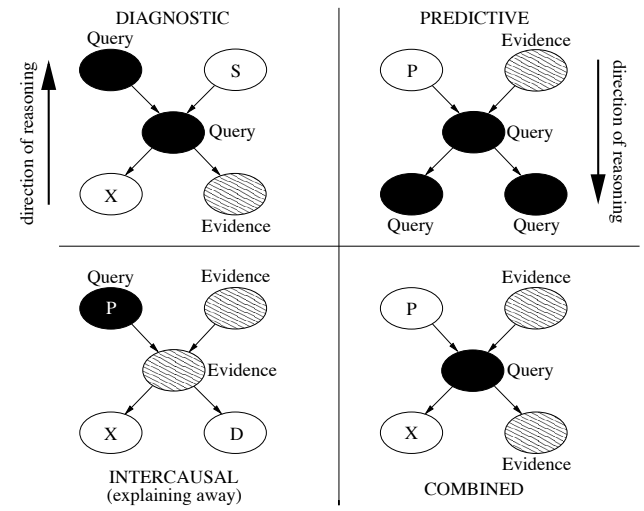
\includegraphics[width=11cm]{fig72.png}
    \centering
    \caption{Tipos de raciocínio presentes em uma rede Bayesiana.}
    \label{fig:fig72}
\end{figure}

\subsection{Estimação de Parâmetros das Redes Bayesianas}

A estimação de parâmetros é a parte final da modelagem por redes bayesianas. Após a seleção das variáveis ter sido feita e a estrutura da rede ter sido fixada, precisamos agora conhecer as probabilidades condicionais de cada variável aleatória, dado os valores de seus antecessores. Para essa tarefa existem várias abordagens. Vamos descrever duas: estimação por máxima verossimilhança (MAP), e estimação por aprendizado sequencial, também conhecida como método bayesiano.

Considerando uma base de dados $D$ completa, e considerando meta-independência global e meta-independência local.

blábláblá...

\subsection{Decisão com Redes Bayesianas}

blábláblá...

\section{Exemplo 1}

\begin{quotation}
Um paciente tem sofrido de falta de ar (dispneia) e visita o médico, preocupado por ter câncer de pulmão. O médico sabe que outras doenças, como tuberculose e bronquite, são possíveis causas, além do câncer de pulmão. Ela também sabe que outras informações relevantes incluem se o paciente é fumante ou não (aumentando as chances de câncer e bronquite) e a que tipo de poluição do ar ele foi exposto. Um raio-X positivo indicaria tuberculose ou câncer de pulmão.
\end{quotation}

\subsection{Definindo os nós e valores}

Primeiro, o engenheiro do conhecimento deve identificar as variáveis ​​de interesse. Isso envolve responder à pergunta: quais são os nós a representar e quais valores eles podem assumir, ou em que estado eles podem estar? Por enquanto, consideraremos apenas os nós que assumem valores discretos. Os valores devem ser mutuamente exclusivos e exaustivos, o que significa que a variável deve assumir exatamente um desses valores por vez. Os tipos comuns de nós discretos incluem:

\begin{itemize}
\item Nós booleanos, que representam proposições, assumindo os valores binários verdadeiro (T) e falso (F). Em um domínio de diagnóstico médico, o nó Câncer representaria a proposição de que um paciente tem câncer.
\item Valores categóricos. Por exemplo, um nó de poluição pode representar a exposição de um paciente à poluição e assumir os valores {baixo, médio, alto}.
\item Valores numéricos. Por exemplo, um nó chamado Idade pode representar a idade de um paciente e ter valores possíveis de 1 a 120.
\end{itemize}

Estratégias podem ser usadas para representar a idade exata de um paciente pode ser agrupar os pacientes em grupos de diferentes idades, como {bebê, criança, adolescente, jovem, meia-idade, velho}. O truque é escolher valores que representem o domínio de forma eficiente, mas com detalhes suficientes para realizar o raciocínio necessário. A Tabela~\ref{tab:tab71} lista as variáveis usadas para análise do caso do câncer de pulmão. 

\begin{table}[t]
    \caption{Escolhas preliminares de nós e valores para o exemplo do câncer de pulmão.}
    \centering
    \begin{tabular}{|c|c|c|}
    \hline
    \textit{Variável} & \textit{Tipo}  & \textit{Valores} \\ \hline
    Poluição & Binário & \{Baixa, Alta\} \\ \hline
    Fumante & Booleano & \{Verdadeiro, Falso\}      \\ \hline
    Câncer & Booleano & \{Verdadeiro, Falso\}      \\ \hline
    Dispnéia & Booleano & \{Verdadeiro, Falso\}      \\ \hline
    Raio-X & Binário  & \{Positivo, Negativo\}  \\ \hline
    \end{tabular}
    \label{tab:tab71}
\end{table}

\subsection{Estrutura}

A estrutura ou topologia da rede deve capturar relacionamentos qualitativos entre as variáveis. Em particular, dois nós devem ser conectados diretamente se um afetar ou causar o outro, com o arco indicando a direção do efeito. Portanto, em nosso exemplo de diagnóstico médico, podemos perguntar quais fatores afetam a chance de um paciente ter câncer? Se a resposta for “Poluição e fumo”, devemos adicionar arcos de Poluição e Fumante a Câncer. Da mesma forma, ter câncer afetará a respiração do paciente e as chances de ter um resultado de raios-X positivo. Portanto, adicionamos arcos de Câncer a Dispneia e Raio-X. A estrutura resultante é mostrada na Figura~\ref{fig:fig72}. É importante notar que esta é apenas uma estrutura possível para o problema; olhamos para estruturas de rede alternativas em

\begin{figure}[t]
    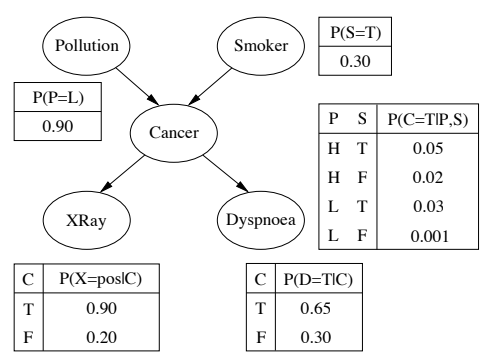
\includegraphics[width=10cm]{fig71.png}
    \centering
    \caption{Uma Rede Bayesiana para o problema do câncer do pulmão.}
    \label{fig:fig72}
\end{figure}

\subsection{Exemplo de código em R e inferência Bayesiana}

A listagem abaixo mostra o código escrito em R. O código utiliza o pacote \textsf{bnlearn} e \textsf{gRain}. A Rede Bayesiana é carregada no formato \textsf{bif} pelo arquivo \textsf{cancer.bif}. As probabilidades marginais de cada nó é representada na Figura~\ref{fig:fig81}

\begin{figure}[t]
    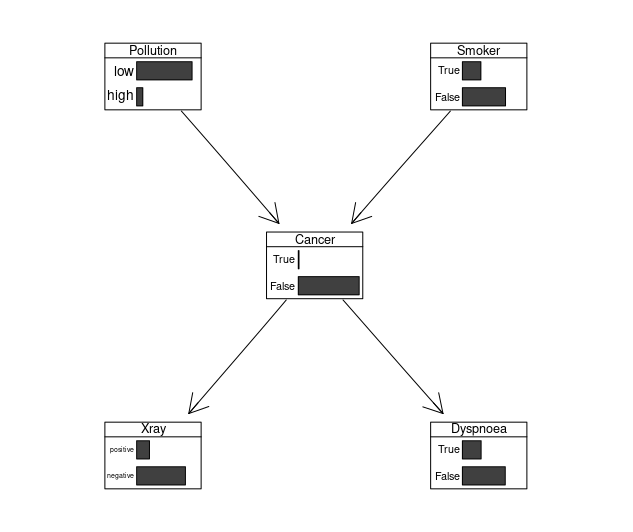
\includegraphics[width=12cm]{fig81.png}
    \centering
    \caption{Probabilidades marginais da rede Bayesiana.}
    \label{fig:fig81}
\end{figure}

São declaradas as evidências \textsf{Pollution = "high"} e \textsf{Xray = "positive"}, ou $Pr(Pollution==high) = 1$ e $Pr(Xray==positive | Cancer==true) = 1$. Consultando a probabilidade posterior antes e depois da declaração das evidências, obtém-se os resultados:

\begin{verbatim}
Cancer
   True   False 
   0.01    0.99 
\end{verbatim}

\begin{verbatim}
Cancer: Pollution = high, Xray = positive.
   True   False 
   0.12    0.88 
\end{verbatim}

Nota-se que a probabilidade de câncer de pulmão elevou de 0,01 para 0,12, dada as evidências.

\lstinputlisting[language=Octave]{code/exemplo1.r}

\end{document}